\section{Methodology}
\label{sec:methodology}

\subsection{Data collection}
Tor has many years' worth of RSA public keys from thousands of Tor relays. The first step I took was to use CollecTor, the Tor network data-collecting service, to collect all recent and archived relay server descriptors. Descriptors that were published in the last 72 hours are available as plain text, and archived descriptors covering over 10 years of Tor network history are available as compressed tarballs. Relay server descriptors contain information that relays publish about themselves such as their nickname, fingerprint, IPv4 address, operating system, Tor version, contact information, and most importantly, their signing key and onion key~\cite{collector}. The signing key is the relay's long-term RSA public identity key and the onion-key, also an RSA public key, is used for short-term encryption. I used the Tor Stem Python controller library to collect all 3,763,821 RSA public keys (signing and onion) from the CollecTor repository of recent and archived server descriptors. It took less than 24 hours to unpack an estimated 200 GB worth of compressed archived relay server descriptor tarballs on a Princeton University computer science departmental machine. The machines used in this paper are all Fujitsu RX200 S8 servers with dual, eight-core 2.8GHz Intel Xeon E5 2680 v2 processors with 256GB RAM running the Springdale distribution of Linux~\cite{cscycles}.

During the key collection process, I serialized a Python dictionary that maps Tor RSA public keys to their relay descriptor metadata. I kept track of each key's relay nickname, identity key fingerprint, time when the descriptor was made, IPv4 address, onion routing port, operating system, tor version, contact information, average bandwidth, and hex encoded digest of extra information. I used this dictionary during my post-fastgcd weak key analysis (see Figure~\ref{rsa-relay}.

\begin{figure}[h]
\centering
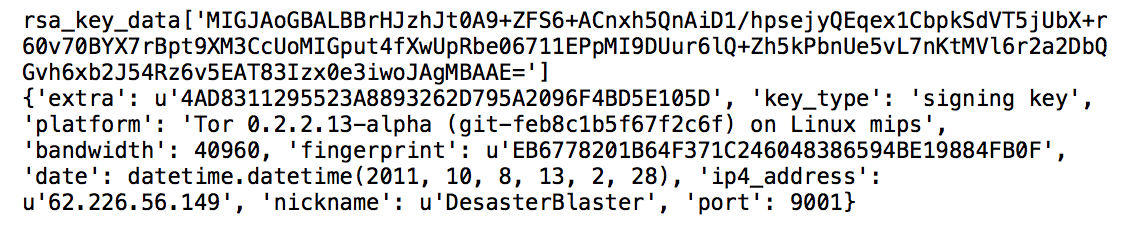
\includegraphics[width=\linewidth]{rsa-relay.png}
\caption{Tor RSA key metadata}
\label{rsa-relay}
\end{figure}

\subsection{Run fastgcd}
To detect potentially weak factorable keys in Tor, I used~\cite{heninger2012mining}'s fastgcd solution for efficiently computing the pair-wise GCD of 3,763,821 Tor public keys generated between December 2005 and December 2016. Fastgcd is a C implementation of an efficient quasilinear-time algorithm for factoring a collection of integers into co-primes. The algorithm is based on Bernstein's algorithm~\cite{bernstein2004find}. As input, fastgcd takes in a file containing a list of RSA moduli in hex. The algorithm computes the GCD of each input integer with the product of every other input integer and outputs two files. One file contains the list of input moduli that had a nontrivial common divisor with any input modulus, and the other file contains the list of common divisors of each vulnerable modulus. 

Before running the set of 3,763,821 RSA public keys through fastgcd, I had to run a few pre-processing steps. To properly extract the moduli from the public keys and convert them to hex, I had to find the lengths and encodings used for the signing and onion keys. After some investigation, I deduced that the Tor RSA keys are 1024-bit, PKCS\#1-padded, OpenSSL PEM-encoded keys~\cite{torspecbug}. The keys returned by Stem are pure RsaPublicKey objects comprised of a base64 ASN.1 sequence with two integers: a modulus N and exponent e. With this knowledge, I was able to use the PyCrypto Python package to properly extract the moduli and exponents from all Tor RSA public key as well as convert the moduli to hex. I ran fastgcd on this pre-processed list of 3,763,821 unique moduli. The program took less than 48 hours to run on Princeton's supercomputers.